% Options for packages loaded elsewhere
\PassOptionsToPackage{unicode}{hyperref}
\PassOptionsToPackage{hyphens}{url}
%
\documentclass[
  english,
  man]{apa6}
\title{EDLD 640 Capstone}
\author{Diana DeWald\textsuperscript{1} \& Dare Baldwin\textsuperscript{1}}
\date{}

\usepackage{amsmath,amssymb}
\usepackage{lmodern}
\usepackage{iftex}
\ifPDFTeX
  \usepackage[T1]{fontenc}
  \usepackage[utf8]{inputenc}
  \usepackage{textcomp} % provide euro and other symbols
\else % if luatex or xetex
  \usepackage{unicode-math}
  \defaultfontfeatures{Scale=MatchLowercase}
  \defaultfontfeatures[\rmfamily]{Ligatures=TeX,Scale=1}
\fi
% Use upquote if available, for straight quotes in verbatim environments
\IfFileExists{upquote.sty}{\usepackage{upquote}}{}
\IfFileExists{microtype.sty}{% use microtype if available
  \usepackage[]{microtype}
  \UseMicrotypeSet[protrusion]{basicmath} % disable protrusion for tt fonts
}{}
\makeatletter
\@ifundefined{KOMAClassName}{% if non-KOMA class
  \IfFileExists{parskip.sty}{%
    \usepackage{parskip}
  }{% else
    \setlength{\parindent}{0pt}
    \setlength{\parskip}{6pt plus 2pt minus 1pt}}
}{% if KOMA class
  \KOMAoptions{parskip=half}}
\makeatother
\usepackage{xcolor}
\IfFileExists{xurl.sty}{\usepackage{xurl}}{} % add URL line breaks if available
\IfFileExists{bookmark.sty}{\usepackage{bookmark}}{\usepackage{hyperref}}
\hypersetup{
  pdftitle={EDLD 640 Capstone},
  pdfauthor={Diana DeWald1 \& Dare Baldwin1},
  pdflang={en-EN},
  pdfkeywords={causal learning models, pedagogy, text analysis},
  hidelinks,
  pdfcreator={LaTeX via pandoc}}
\urlstyle{same} % disable monospaced font for URLs
\usepackage{color}
\usepackage{fancyvrb}
\newcommand{\VerbBar}{|}
\newcommand{\VERB}{\Verb[commandchars=\\\{\}]}
\DefineVerbatimEnvironment{Highlighting}{Verbatim}{commandchars=\\\{\}}
% Add ',fontsize=\small' for more characters per line
\usepackage{framed}
\definecolor{shadecolor}{RGB}{248,248,248}
\newenvironment{Shaded}{\begin{snugshade}}{\end{snugshade}}
\newcommand{\AlertTok}[1]{\textcolor[rgb]{0.94,0.16,0.16}{#1}}
\newcommand{\AnnotationTok}[1]{\textcolor[rgb]{0.56,0.35,0.01}{\textbf{\textit{#1}}}}
\newcommand{\AttributeTok}[1]{\textcolor[rgb]{0.77,0.63,0.00}{#1}}
\newcommand{\BaseNTok}[1]{\textcolor[rgb]{0.00,0.00,0.81}{#1}}
\newcommand{\BuiltInTok}[1]{#1}
\newcommand{\CharTok}[1]{\textcolor[rgb]{0.31,0.60,0.02}{#1}}
\newcommand{\CommentTok}[1]{\textcolor[rgb]{0.56,0.35,0.01}{\textit{#1}}}
\newcommand{\CommentVarTok}[1]{\textcolor[rgb]{0.56,0.35,0.01}{\textbf{\textit{#1}}}}
\newcommand{\ConstantTok}[1]{\textcolor[rgb]{0.00,0.00,0.00}{#1}}
\newcommand{\ControlFlowTok}[1]{\textcolor[rgb]{0.13,0.29,0.53}{\textbf{#1}}}
\newcommand{\DataTypeTok}[1]{\textcolor[rgb]{0.13,0.29,0.53}{#1}}
\newcommand{\DecValTok}[1]{\textcolor[rgb]{0.00,0.00,0.81}{#1}}
\newcommand{\DocumentationTok}[1]{\textcolor[rgb]{0.56,0.35,0.01}{\textbf{\textit{#1}}}}
\newcommand{\ErrorTok}[1]{\textcolor[rgb]{0.64,0.00,0.00}{\textbf{#1}}}
\newcommand{\ExtensionTok}[1]{#1}
\newcommand{\FloatTok}[1]{\textcolor[rgb]{0.00,0.00,0.81}{#1}}
\newcommand{\FunctionTok}[1]{\textcolor[rgb]{0.00,0.00,0.00}{#1}}
\newcommand{\ImportTok}[1]{#1}
\newcommand{\InformationTok}[1]{\textcolor[rgb]{0.56,0.35,0.01}{\textbf{\textit{#1}}}}
\newcommand{\KeywordTok}[1]{\textcolor[rgb]{0.13,0.29,0.53}{\textbf{#1}}}
\newcommand{\NormalTok}[1]{#1}
\newcommand{\OperatorTok}[1]{\textcolor[rgb]{0.81,0.36,0.00}{\textbf{#1}}}
\newcommand{\OtherTok}[1]{\textcolor[rgb]{0.56,0.35,0.01}{#1}}
\newcommand{\PreprocessorTok}[1]{\textcolor[rgb]{0.56,0.35,0.01}{\textit{#1}}}
\newcommand{\RegionMarkerTok}[1]{#1}
\newcommand{\SpecialCharTok}[1]{\textcolor[rgb]{0.00,0.00,0.00}{#1}}
\newcommand{\SpecialStringTok}[1]{\textcolor[rgb]{0.31,0.60,0.02}{#1}}
\newcommand{\StringTok}[1]{\textcolor[rgb]{0.31,0.60,0.02}{#1}}
\newcommand{\VariableTok}[1]{\textcolor[rgb]{0.00,0.00,0.00}{#1}}
\newcommand{\VerbatimStringTok}[1]{\textcolor[rgb]{0.31,0.60,0.02}{#1}}
\newcommand{\WarningTok}[1]{\textcolor[rgb]{0.56,0.35,0.01}{\textbf{\textit{#1}}}}
\usepackage{graphicx}
\makeatletter
\def\maxwidth{\ifdim\Gin@nat@width>\linewidth\linewidth\else\Gin@nat@width\fi}
\def\maxheight{\ifdim\Gin@nat@height>\textheight\textheight\else\Gin@nat@height\fi}
\makeatother
% Scale images if necessary, so that they will not overflow the page
% margins by default, and it is still possible to overwrite the defaults
% using explicit options in \includegraphics[width, height, ...]{}
\setkeys{Gin}{width=\maxwidth,height=\maxheight,keepaspectratio}
% Set default figure placement to htbp
\makeatletter
\def\fps@figure{htbp}
\makeatother
\setlength{\emergencystretch}{3em} % prevent overfull lines
\providecommand{\tightlist}{%
  \setlength{\itemsep}{0pt}\setlength{\parskip}{0pt}}
\setcounter{secnumdepth}{-\maxdimen} % remove section numbering
% Make \paragraph and \subparagraph free-standing
\ifx\paragraph\undefined\else
  \let\oldparagraph\paragraph
  \renewcommand{\paragraph}[1]{\oldparagraph{#1}\mbox{}}
\fi
\ifx\subparagraph\undefined\else
  \let\oldsubparagraph\subparagraph
  \renewcommand{\subparagraph}[1]{\oldsubparagraph{#1}\mbox{}}
\fi
\newlength{\cslhangindent}
\setlength{\cslhangindent}{1.5em}
\newlength{\csllabelwidth}
\setlength{\csllabelwidth}{3em}
\newlength{\cslentryspacingunit} % times entry-spacing
\setlength{\cslentryspacingunit}{\parskip}
\newenvironment{CSLReferences}[2] % #1 hanging-ident, #2 entry spacing
 {% don't indent paragraphs
  \setlength{\parindent}{0pt}
  % turn on hanging indent if param 1 is 1
  \ifodd #1
  \let\oldpar\par
  \def\par{\hangindent=\cslhangindent\oldpar}
  \fi
  % set entry spacing
  \setlength{\parskip}{#2\cslentryspacingunit}
 }%
 {}
\usepackage{calc}
\newcommand{\CSLBlock}[1]{#1\hfill\break}
\newcommand{\CSLLeftMargin}[1]{\parbox[t]{\csllabelwidth}{#1}}
\newcommand{\CSLRightInline}[1]{\parbox[t]{\linewidth - \csllabelwidth}{#1}\break}
\newcommand{\CSLIndent}[1]{\hspace{\cslhangindent}#1}
% Manuscript styling
\usepackage{upgreek}
\captionsetup{font=singlespacing,justification=justified}

% Table formatting
\usepackage{longtable}
\usepackage{lscape}
% \usepackage[counterclockwise]{rotating}   % Landscape page setup for large tables
\usepackage{multirow}		% Table styling
\usepackage{tabularx}		% Control Column width
\usepackage[flushleft]{threeparttable}	% Allows for three part tables with a specified notes section
\usepackage{threeparttablex}            % Lets threeparttable work with longtable

% Create new environments so endfloat can handle them
% \newenvironment{ltable}
%   {\begin{landscape}\centering\begin{threeparttable}}
%   {\end{threeparttable}\end{landscape}}
\newenvironment{lltable}{\begin{landscape}\centering\begin{ThreePartTable}}{\end{ThreePartTable}\end{landscape}}

% Enables adjusting longtable caption width to table width
% Solution found at http://golatex.de/longtable-mit-caption-so-breit-wie-die-tabelle-t15767.html
\makeatletter
\newcommand\LastLTentrywidth{1em}
\newlength\longtablewidth
\setlength{\longtablewidth}{1in}
\newcommand{\getlongtablewidth}{\begingroup \ifcsname LT@\roman{LT@tables}\endcsname \global\longtablewidth=0pt \renewcommand{\LT@entry}[2]{\global\advance\longtablewidth by ##2\relax\gdef\LastLTentrywidth{##2}}\@nameuse{LT@\roman{LT@tables}} \fi \endgroup}

% \setlength{\parindent}{0.5in}
% \setlength{\parskip}{0pt plus 0pt minus 0pt}

% \usepackage{etoolbox}
\makeatletter
\patchcmd{\HyOrg@maketitle}
  {\section{\normalfont\normalsize\abstractname}}
  {\section*{\normalfont\normalsize\abstractname}}
  {}{\typeout{Failed to patch abstract.}}
\patchcmd{\HyOrg@maketitle}
  {\section{\protect\normalfont{\@title}}}
  {\section*{\protect\normalfont{\@title}}}
  {}{\typeout{Failed to patch title.}}
\makeatother
\shorttitle{Natural Language Processing for Pedagogy}
\keywords{causal learning models, pedagogy, text analysis\newline\indent Word count: 1219}
\DeclareDelayedFloatFlavor{ThreePartTable}{table}
\DeclareDelayedFloatFlavor{lltable}{table}
\DeclareDelayedFloatFlavor*{longtable}{table}
\makeatletter
\renewcommand{\efloat@iwrite}[1]{\immediate\expandafter\protected@write\csname efloat@post#1\endcsname{}}
\makeatother
\usepackage{lineno}

\linenumbers
\usepackage{csquotes}
\ifXeTeX
  % Load polyglossia as late as possible: uses bidi with RTL langages (e.g. Hebrew, Arabic)
  \usepackage{polyglossia}
  \setmainlanguage[]{english}
\else
  \usepackage[main=english]{babel}
% get rid of language-specific shorthands (see #6817):
\let\LanguageShortHands\languageshorthands
\def\languageshorthands#1{}
\fi
\ifLuaTeX
  \usepackage{selnolig}  % disable illegal ligatures
\fi


\affiliation{\vspace{0.5cm}\textsuperscript{1} University of Oregon}

\abstract{
How is young children's exploration impacted by adult pedagogy? Can we create Machine Learning models to predict how a child will explore the causal features of an object based upon the pedagogy they are exposed to? Our goal is to establish predictive models of preschoolers' causal learning outcomes within educational settings based upon teachers' pedagogical styles. Using pre-existing samples of pedagogy and child outcomes, we created three machine learning models to capture 1) the extent to which adults produce pedagogy that is likely to have the intended effect on preschoolers' play behavior when prompted accordingly, and 2) the extent to which pedagogy that has different intent based upon the prompt differs in sentiment. We found that\ldots\ldots{}
}



\begin{document}
\maketitle

\hypertarget{introduction}{%
\section{Introduction}\label{introduction}}

Developmentalists and educators have long debated the benefits of child-directed (Montessori style) exploration contra adult-directed (pedagogical) instruction on learning outcomes. While young children (age 3-6) often re-structure their hypotheses about the world based upon self-directed exploration á la Montessori, there are many subjects children cannot master without adult-directed pedagogical guidance (e.g., novel object labels, the alphabet, color and shape labels, historical events, the existence of entities such as germs, etc.). Such subjects are often culturally and linguistically bound, but even causal learning related to the physical properties of objects and entities can benefit from adult-directed pedagogy. Clarifying the extent to which pedagogy supports---and in some cases diminishes---effective causal learning is essential for a) informing teaching strategies in a time when many preparatory schools in the U.S. suffer from a lack of funding and teacher support (\textbf{SRCD?}; \textbf{NIERR?}), and b) elevating early education outcomes following relative dips in school preparedness over the past three years (Jalongo, 2021; (\textbf{gonzalez2022school?})).
Those who have sought to address the impact of adult-directed pedagogy on causal learning describe a pedagogical trade-off model. This model proposes that adult instruction increases the proportion of time children spend exploring an object's pedagogy-relevant properties but limits their investigation of other properties. Conversely, child-directed exploration is understood to produce broader discovery of the complete set of an object's causal properties but diminish the time spent investigating any particular property.While such behavioral outcomes are established, little is known about the differential impact of diverse pedagogy types (such method tend to rely on one pedagogical condition statement, usually ``This is how my toy works'').
In this project, we were interested in the relation between adults' use of language while teaching and children's learning outcomes. Specifically, we wanted to investigate how diverse and naturalistic pedagogy types that were produced to encourage children's play based upon findings from the pedagogy trade-off model would align with the pedagogy utilized within typical empirical methods for this model. To examine this, we took pre-existing text data from a survey where we asked UO students to watch a video depicting a toy and generate a text response detailing how they would go about teaching a preschooler about the toy. In one between subjects condition, they were instructed to `enhance' exploration (i.e., by providing pedagogy that would encourage a child to explore beyond one object property). In a second condition, they were instructed to `constrain exploration (i.e., by providing pedagogy that would encourage a child to only explore the one property demonstrated in the video).
After presenting descriptives on the survey text dataset, we go on to describe three machine learning models to investigate different aims. The first model was created to predict the likelihood of a positive or negative sentiment occurring based upon the condition (enhance or constrain), source (qualtrics survey or pre-existing study pedagogy) and function (we included both a 'squeaker' and a `light' function in the object introduction video). The second model was created to predict the distance among expected outcomes paired via a manual coding system to the pedagogy samples from the survey (K-nearest neighbors). The third model again used logistic regression to create a best-performing model predicting child play outcomes (we collected in Fall of 2022 at the Oregon Museum of Science and Industry) from 4 pedagogy types used in that method.

\hypertarget{methods}{%
\section{Methods}\label{methods}}

\begin{verbatim}
In Fall of 2022, we conducted a Qualtrics survey of undergraduate students 
\end{verbatim}

(N = 168) at the University of Oregon, asking participants to report how they
would teach a child about the causal properties of a novel object. Participants
were randomly sorted into 2 conditions. In the `enhance' condition, participants
were instructed to generate pedagogy for two object properties with the intention
to produce broad exploratory behaviors from a child (prompt: ``what would you say )
to intoduce this toy in a way that encourages wide-ranging exploration?''). In the
`constrain' condition, participants were asked to generate pedagogy intended to
produce limited exploratory behaviors from a child (prompt: ``What would you say )
to introduce this toy in a way that discourages wide-ranging exploration?''). We
subsequently assessed overall word frequencies, and word frequencies by condition
(see `Results: Descriptive Plots'). Next, we investigated the extent to which the
`constrain' pedagogy differed in sentiment from the `enhance' pedagogy (see\\
`Results: Model 1')
In Model 2, we utilized a coding classifier system pairing
participant-generated pedagogy with 7 pedagogy-type categories from previous
research. These 7 pedagogy categories were linked to specific child outcomes from
prior studies conducted by us as well as other labs. See Results: Model 2 for the
model performance. Finally, using child data outcome data from our lab, we created
a model to predict child outcomes based upon four pedagogy types from that study
(Model 3). Having previously paired these four pedagogy types with items on the
7-point scale, this gives us the ability to indirectly assess the likelihood that
the survey-generated pedagogy text data will produce the desired child outcomes.

\hypertarget{results-descriptive-plots-word-counts}{%
\section{Results: Descriptive plots (word counts)}\label{results-descriptive-plots-word-counts}}

\begin{Shaded}
\begin{Highlighting}[]
\CommentTok{\# parsing words from the \textquotesingle{}pedagogy\textquotesingle{} (text) column}
\NormalTok{tidy\_words }\OtherTok{\textless{}{-}}\NormalTok{ mydata }\SpecialCharTok{\%\textgreater{}\%}
  \FunctionTok{unnest\_tokens}\NormalTok{(word, pedagogy)}

\CommentTok{\# removing numbers}
\NormalTok{tidy\_words }\OtherTok{\textless{}{-}}\NormalTok{ tidy\_words[}\SpecialCharTok{{-}}\FunctionTok{grep}\NormalTok{(}\StringTok{"}\SpecialCharTok{\textbackslash{}\textbackslash{}}\StringTok{b}\SpecialCharTok{\textbackslash{}\textbackslash{}}\StringTok{d+}\SpecialCharTok{\textbackslash{}\textbackslash{}}\StringTok{b"}\NormalTok{, tidy\_words}\SpecialCharTok{$}\NormalTok{word),]}

\CommentTok{\# removing common/under{-}informative words}
\NormalTok{exclu }\OtherTok{\textless{}{-}} \FunctionTok{tibble}\NormalTok{(}\AttributeTok{word =} \FunctionTok{c}\NormalTok{(}\StringTok{"the"}\NormalTok{, }\StringTok{"this"}\NormalTok{, }\StringTok{"I"}\NormalTok{))}

\NormalTok{tidy\_words }\OtherTok{\textless{}{-}}\NormalTok{ tidy\_words }\SpecialCharTok{\%\textgreater{}\%}
  \FunctionTok{anti\_join}\NormalTok{(exclu, }\AttributeTok{by =} \StringTok{"word"}\NormalTok{)}


\CommentTok{\#plot}
\NormalTok{tidy\_words }\SpecialCharTok{\%\textgreater{}\%} 
  \FunctionTok{anti\_join}\NormalTok{(stop\_words) }\SpecialCharTok{\%\textgreater{}\%} 
  \FunctionTok{count}\NormalTok{(word, }\AttributeTok{sort =} \ConstantTok{TRUE}\NormalTok{) }\SpecialCharTok{\%\textgreater{}\%} 
  \FunctionTok{mutate}\NormalTok{(}\AttributeTok{word =} \FunctionTok{reorder}\NormalTok{(word, n)) }\SpecialCharTok{\%\textgreater{}\%} \CommentTok{\# make y{-}axis ordered by n}
  \FunctionTok{slice}\NormalTok{(}\DecValTok{1}\SpecialCharTok{:}\DecValTok{15}\NormalTok{) }\SpecialCharTok{\%\textgreater{}\%} \CommentTok{\# select only the first 15 rows}
  \FunctionTok{ggplot}\NormalTok{(}\FunctionTok{aes}\NormalTok{(n, word)) }\SpecialCharTok{+}
  \FunctionTok{geom\_col}\NormalTok{(}\AttributeTok{fill =} \StringTok{"royalblue"}\NormalTok{, }\AttributeTok{alpha =}\NormalTok{ .}\DecValTok{7}\NormalTok{) }\SpecialCharTok{+}
  \FunctionTok{scale\_x\_continuous}\NormalTok{(}\AttributeTok{expand =} \FunctionTok{c}\NormalTok{(}\DecValTok{0}\NormalTok{,}\DecValTok{0}\NormalTok{)) }\SpecialCharTok{+}
  \FunctionTok{theme\_minimal}\NormalTok{() }\SpecialCharTok{+}
  \FunctionTok{theme}\NormalTok{(}
    \AttributeTok{panel.grid.major.y =} \FunctionTok{element\_blank}\NormalTok{(),}
    \AttributeTok{panel.grid.minor.x =} \FunctionTok{element\_blank}\NormalTok{(),}
    \AttributeTok{panel.grid.major.x =} \FunctionTok{element\_line}\NormalTok{(}\AttributeTok{color =} \StringTok{"gray80"}\NormalTok{)}
\NormalTok{  ) }\SpecialCharTok{+}
  \FunctionTok{labs}\NormalTok{(}
    \AttributeTok{x =} \StringTok{"Word Frequency"}\NormalTok{,}
    \AttributeTok{y =} \StringTok{"Word"}\NormalTok{,}
    \AttributeTok{title =} \StringTok{"Figure 1: Top 15 most frequently occurring words across all pedagogy types"}\NormalTok{,}
\NormalTok{  )}
\end{Highlighting}
\end{Shaded}

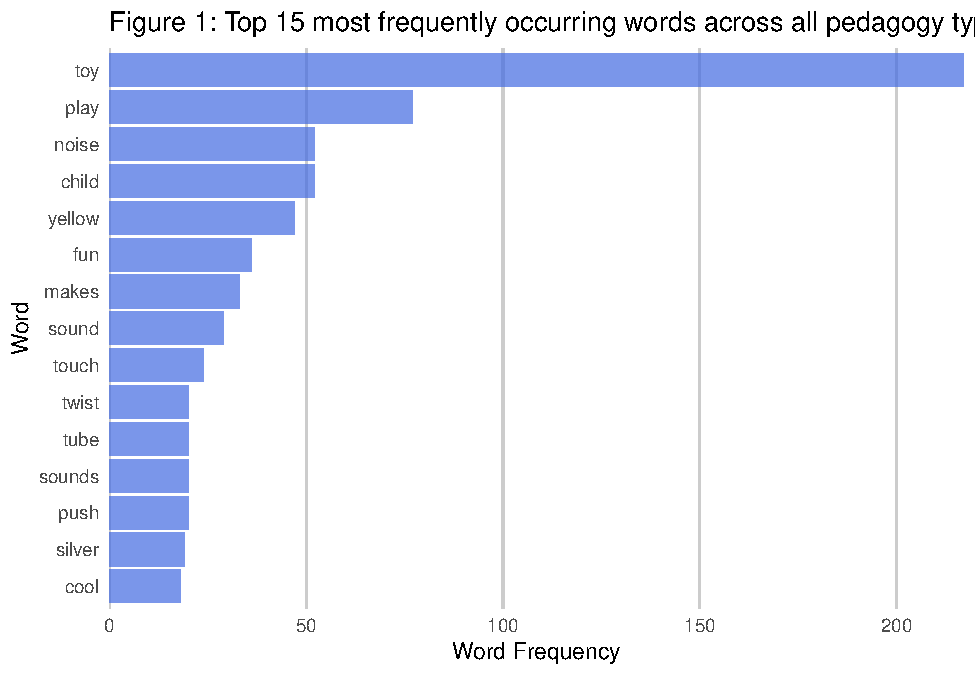
\includegraphics{capstone640_files/figure-latex/initial plots-1.pdf}

\hypertarget{figure-2-word-frequency-cloud-across-conditions}{%
\section{Figure 2: Word Frequency Cloud (Across Conditions)}\label{figure-2-word-frequency-cloud-across-conditions}}

\begin{Shaded}
\begin{Highlighting}[]
\CommentTok{\# visualing: word cloud}
\FunctionTok{library}\NormalTok{(wordcloud)}

\NormalTok{tokens }\OtherTok{=}\NormalTok{ textdata }\SpecialCharTok{\%\textgreater{}\%}
  \FunctionTok{unnest\_tokens}\NormalTok{(word, text) }\SpecialCharTok{\%\textgreater{}\%}
  \FunctionTok{anti\_join}\NormalTok{(stop\_words)}

\CommentTok{\# top words}
\NormalTok{word\_count }\OtherTok{=}\NormalTok{ tokens}\SpecialCharTok{\%\textgreater{}\%}
  \FunctionTok{group\_by}\NormalTok{(word)}\SpecialCharTok{\%\textgreater{}\%}
  \FunctionTok{summarise}\NormalTok{(}\AttributeTok{count =} \FunctionTok{n}\NormalTok{())}\SpecialCharTok{\%\textgreater{}\%}
  \FunctionTok{arrange}\NormalTok{(}\FunctionTok{desc}\NormalTok{(count))}\SpecialCharTok{\%\textgreater{}\%}
  \FunctionTok{slice}\NormalTok{(}\DecValTok{1}\SpecialCharTok{:}\DecValTok{10}\NormalTok{)}


\CommentTok{\# word cloud{-}{-}zoom in}
\NormalTok{cloud }\OtherTok{\textless{}{-}}\NormalTok{ tokens }\SpecialCharTok{\%\textgreater{}\%}
  \FunctionTok{group\_by}\NormalTok{(source, word) }\SpecialCharTok{\%\textgreater{}\%}
  \FunctionTok{summarise}\NormalTok{(}\AttributeTok{count =} \FunctionTok{n}\NormalTok{())}\SpecialCharTok{\%\textgreater{}\%}
  \FunctionTok{arrange}\NormalTok{(}\FunctionTok{desc}\NormalTok{(count))}\SpecialCharTok{\%\textgreater{}\%}
  \FunctionTok{slice}\NormalTok{(}\DecValTok{1}\SpecialCharTok{:}\DecValTok{10}\NormalTok{)}
  

\FunctionTok{wordcloud}\NormalTok{(tokens}\SpecialCharTok{$}\NormalTok{word, }\AttributeTok{max.words =} \DecValTok{75}\NormalTok{, }\AttributeTok{colors=}\FunctionTok{brewer.pal}\NormalTok{(}\DecValTok{6}\NormalTok{, }\StringTok{"Dark2"}\NormalTok{))}
\end{Highlighting}
\end{Shaded}

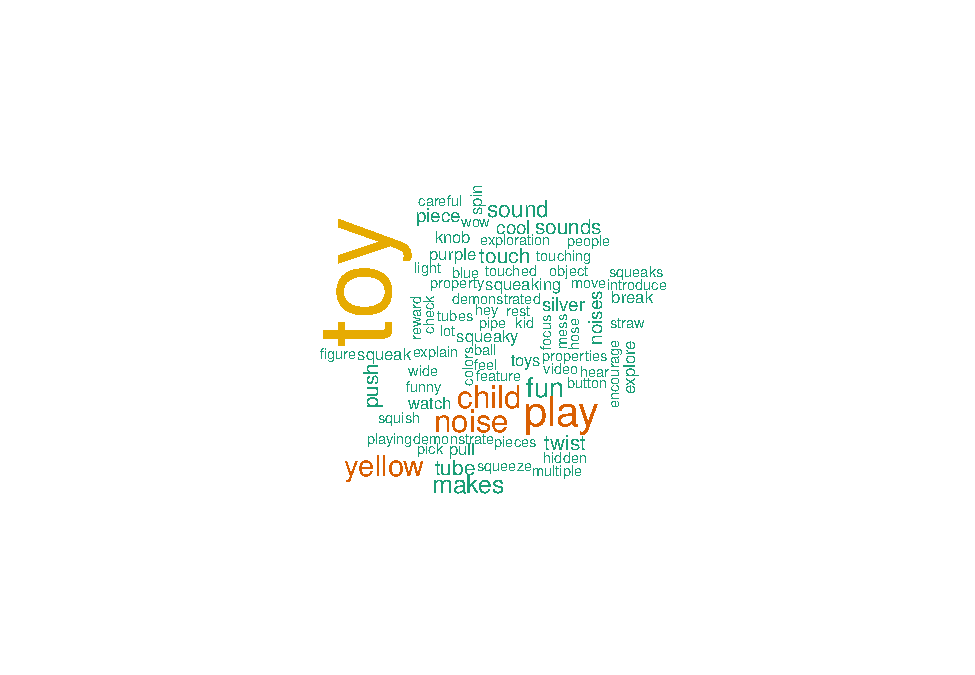
\includegraphics{capstone640_files/figure-latex/word cloud-1.pdf}

\begin{Shaded}
\begin{Highlighting}[]
\NormalTok{tidy\_words }\SpecialCharTok{\%\textgreater{}\%} 
  \FunctionTok{group\_by}\NormalTok{(condition) }\SpecialCharTok{\%\textgreater{}\%}
  \FunctionTok{anti\_join}\NormalTok{(stop\_words) }\SpecialCharTok{\%\textgreater{}\%} 
  \FunctionTok{count}\NormalTok{(word, }\AttributeTok{sort =} \ConstantTok{TRUE}\NormalTok{) }\SpecialCharTok{\%\textgreater{}\%} 
  \FunctionTok{mutate}\NormalTok{(}\AttributeTok{word =} \FunctionTok{reorder}\NormalTok{(word, n)) }\SpecialCharTok{\%\textgreater{}\%} \CommentTok{\# make y{-}axis ordered by n}
  \FunctionTok{slice}\NormalTok{(}\DecValTok{1}\SpecialCharTok{:}\DecValTok{15}\NormalTok{) }\SpecialCharTok{\%\textgreater{}\%} \CommentTok{\# select only the first 15 rows}
  \FunctionTok{ggplot}\NormalTok{(}\FunctionTok{aes}\NormalTok{(n, word, }\AttributeTok{fill =}\NormalTok{ condition)) }\SpecialCharTok{+}
  \FunctionTok{geom\_col}\NormalTok{(}\AttributeTok{alpha =}\NormalTok{ .}\DecValTok{7}\NormalTok{) }\SpecialCharTok{+}
  \FunctionTok{facet\_wrap}\NormalTok{(}\SpecialCharTok{\textasciitilde{}}\NormalTok{condition) }\SpecialCharTok{+}
  \FunctionTok{scale\_x\_continuous}\NormalTok{(}\AttributeTok{expand =} \FunctionTok{c}\NormalTok{(}\DecValTok{0}\NormalTok{,}\DecValTok{0}\NormalTok{)) }\SpecialCharTok{+}
  \FunctionTok{theme\_minimal}\NormalTok{() }\SpecialCharTok{+}
  \FunctionTok{theme}\NormalTok{(}
    \AttributeTok{panel.grid.major.y =} \FunctionTok{element\_blank}\NormalTok{(),}
    \AttributeTok{panel.grid.minor.x =} \FunctionTok{element\_blank}\NormalTok{(),}
    \AttributeTok{panel.grid.major.x =} \FunctionTok{element\_line}\NormalTok{(}\AttributeTok{color =} \StringTok{"gray80"}\NormalTok{)}
\NormalTok{  ) }\SpecialCharTok{+}
  \FunctionTok{labs}\NormalTok{(}
    \AttributeTok{x =} \StringTok{"Word Frequency"}\NormalTok{,}
    \AttributeTok{y =} \StringTok{"Word"}\NormalTok{,}
    \AttributeTok{title =} \StringTok{"Figure 3: Top 15 most frequently occurring words by condition"}\NormalTok{,}
\NormalTok{  )}
\end{Highlighting}
\end{Shaded}

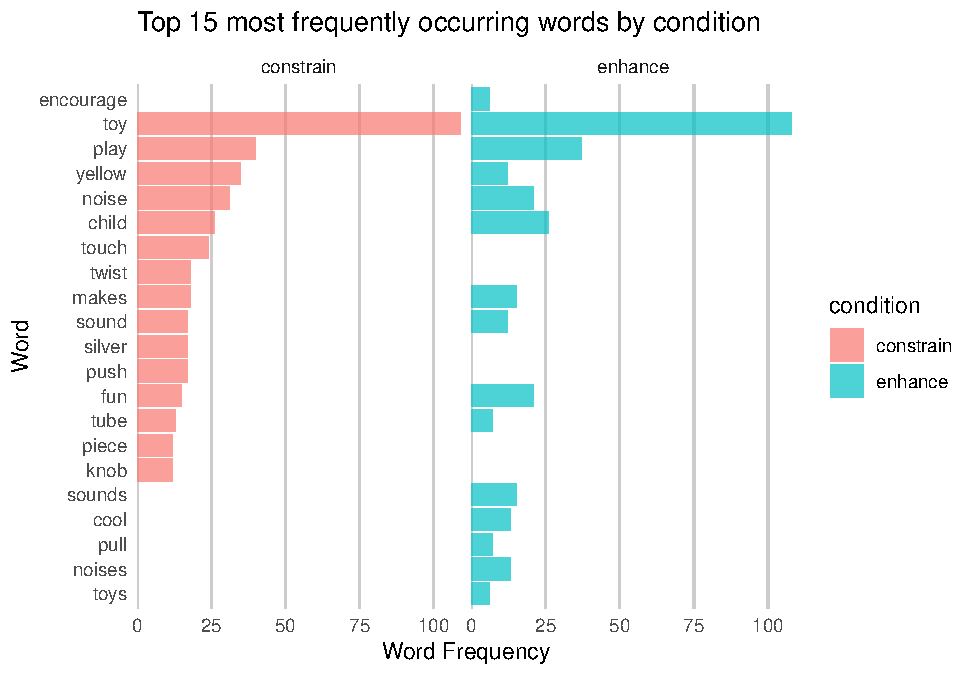
\includegraphics{capstone640_files/figure-latex/unnamed-chunk-1-1.pdf}
In Figure 3, we see the top 15 words used in the enhance and constrain
conditions. In the `enahnce' condition, there was greater use of words like ``sounds,'' ``cool,'' ``pull,'' ``noises,'' and ``toys.'' In the `constrain' condition, there was greater use of ``touch,'' ``silver,'' ``push,'' and ``knob.''

\hypertarget{description-of-sentiment-analysis}{%
\subsubsection{Description of sentiment analysis}\label{description-of-sentiment-analysis}}

\begin{table}

\caption{\label{tab:unnamed-chunk-3}Sentiment by analysis tool}
\centering
\begin{threeparttable}
\begin{tabular}[t]{>{\raggedleft\arraybackslash}p{0.57in}|>{\raggedleft\arraybackslash}p{0.57in}|>{\raggedleft\arraybackslash}p{0.57in}|>{\raggedleft\arraybackslash}p{0.57in}|>{\raggedleft\arraybackslash}p{0.57in}|>{\raggedleft\arraybackslash}p{0.57in}|>{\raggedleft\arraybackslash}p{0.57in}|>{\raggedleft\arraybackslash}p{0.57in}|>{\raggedleft\arraybackslash}p{0.57in}|>{\raggedleft\arraybackslash}p{0.57in}}
\hline
Pos bing & Neg bing & Pos nrc & Neg nrc & Pos loughran & Neg loughran & Pos afinn & Neg afinn & Total Positive & Total Negative\\
\hline
64 & 66 & 277 & 73 & 18 & 73 & 61 & 10 & 420 & 222\\
\hline
41 & 116 & 274 & 94 & 40 & 28 & 54 & 26 & 409 & 264\\
\hline
\end{tabular}
\begin{tablenotes}[para]
\item \textit{Note.} 
\item Positive (Pos) and Negative (Neg) sentiment analysis by individual words using 4 analysis tools: bing, nrc, loughran, and afinn. Results demonstrate that Total Positive \& Negative sentiment was roughly equal by condition (enhance or constrain). However, positive sentiment was slightly higher for the enhance condition and negative sentiment was slight higher for the constrain condition, which is the expected result.
\end{tablenotes}
\end{threeparttable}
\end{table}

\hypertarget{model-1-predicting-a-categorical-outcome-sentiment-positive-or-negative-using-regularized-logistic-regression}{%
\subsection{Model 1: Predicting a Categorical Outcome (sentiment: positive or negative) using Regularized Logistic Regression}\label{model-1-predicting-a-categorical-outcome-sentiment-positive-or-negative-using-regularized-logistic-regression}}

\begin{verbatim}
## Generalized Linear Model 
## 
## 230 samples
##   6 predictor
##   2 classes: 'negative', 'positive' 
## 
## Recipe steps: zv 
## Resampling: Cross-Validated (10 fold) 
## Summary of sample sizes: 207, 207, 207, 207, 207, 207, ... 
## Resampling results:
## 
##   logLoss  
##   0.6264822
\end{verbatim}

\begin{verbatim}
##    negative  positive
## 1 0.7771235 0.2228765
## 2 0.5675647 0.4324353
## 3 0.7771235 0.2228765
## 4 0.5675647 0.4324353
## 5 0.5675647 0.4324353
## 6 0.7771235 0.2228765
\end{verbatim}

\begin{verbatim}
## [1] 0.02639752
\end{verbatim}

\begin{verbatim}
## [1] 0.6140351
\end{verbatim}

\begin{verbatim}
## [1] 0.7836039
\end{verbatim}

\hypertarget{results-model-1}{%
\section{Results Model 1}\label{results-model-1}}

The first model is a regularized logistic regression predicting sentiment type (positive or negative) from a participant's condition (enhance or constrain), source (qualtrics survey or pre-existing study pedagogy) and function (`squeaker' or 'light). Results indicate that pedagogy did not differ significantly in sentiment based upon the condition participants were in\ldots{} Model performance\ldots.

\hypertarget{model-2-k-nearest-neighbors}{%
\subsubsection{Model 2: K-nearest neighbors}\label{model-2-k-nearest-neighbors}}

\hypertarget{model-3-logistic-regression-predicting-whether-a-particular-object-function-was-discovered}{%
\subsubsection{Model 3: Logistic regression predicting whether a particular object function was discovered}\label{model-3-logistic-regression-predicting-whether-a-particular-object-function-was-discovered}}

\begin{verbatim}
##   parameter   class                    label
## 1     alpha numeric        Mixing Percentage
## 2    lambda numeric Regularization Parameter
\end{verbatim}

The optimal lambda value for a lasso penalty was \_\_\_\_\_

According to the second lasso model, the optimal lambda value for lasso penalty is \_\_\_\_\_\_\_

\hypertarget{find-and-report-the-most-important-10-predictors-of-sentiment-and-their-coefficients.}{%
\subsubsection{Find and report the most important 10 predictors of sentiment and their coefficients.}\label{find-and-report-the-most-important-10-predictors-of-sentiment-and-their-coefficients.}}

\hypertarget{k-nearest-neighbors-algorithm-to-predict-rank-ordered-exploration-promotion}{%
\subsection{K-nearest neighbors algorithm to predict rank ordered exploration-promotion}\label{k-nearest-neighbors-algorithm-to-predict-rank-ordered-exploration-promotion}}

\hypertarget{import-data}{%
\section{import data}\label{import-data}}

textdummy \textless- import(here(``data,'' ``text\_data\_dummy.xlsx''))

\hypertarget{train-and-test-split}{%
\section{train and test split}\label{train-and-test-split}}

set.seed(10152022) \# for reproducibility

loc \textless- sample(1:nrow(textdummy), round(nrow(textdummy) * 0.9))
rank\_tr \textless- textdummy{[}loc, {]}
rank\_te \textless- textdummy{[}-loc, {]}

\hypertarget{create-row-indices-for-10-folds}{%
\section{create row indices for 10-folds}\label{create-row-indices-for-10-folds}}

\#randomly shuffle training data
rank\_tr = rank\_tr{[}sample(nrow(rank\_tr)),{]}

\begin{verbatim}
# Create 10 folds with equal size

  folds = cut(seq(1,nrow(rank_tr)),breaks=10,labels=FALSE)

# Create the list for each fold 
  
  my.indices <- vector('list',10)
  for(i in 1:10){
    my.indices[[i]] <- which(folds!=i)
  }
\end{verbatim}

\hypertarget{cross-validation-settings}{%
\section{Cross-validation settings}\label{cross-validation-settings}}

cv \textless- trainControl(method = ``cv,''
index = my.indices)

require(caret)
require(kknn)

getModelInfo()\(kknn\)parameters

\hypertarget{hyperparameter-tuning-grid}{%
\section{Hyperparameter Tuning Grid}\label{hyperparameter-tuning-grid}}

grid \textless- expand.grid(kmax = 3:25,
distance = c(1,2,3),
kernel = c(`epanechnikov,'`rectangular'))
grid

require(doParallel)

ncores \textless- 8

cl \textless- makePSOCKcluster(ncores)

registerDoParallel(cl)

\hypertarget{train-the-model}{%
\section{Train the model}\label{train-the-model}}

outcome \textless- c(`rank')

ID \textless- c(`id')

categorical \textless- c(`condition,' `source,' `function')

blueprint\_textdummy \textless- recipe(x = textdummy,
vars = c(categorical, outcome, ID),
roles = c(rep(`predictor,'3), `outcome,' `ID'))

caret\_knn \textless- caret::train(blueprint\_textdummy,
data = rank\_tr,
method = ``kknn,''
trControl = cv,
tuneGrid = grid)

\hypertarget{results-model-2}{%
\section{Results Model 2}\label{results-model-2}}

\hypertarget{results-model-3}{%
\section{Results Model 3}\label{results-model-3}}

\hypertarget{discussion-in-progress}{%
\section{Discussion (in progress)}\label{discussion-in-progress}}

\newpage

\hypertarget{references}{%
\section{References}\label{references}}

We used packages from R {[}Version 4.1.1; R Core Team (2021){]} and the R-package \emph{papaja} {[}Version 0.1.0.9997; Aust and Barth (2020){]} for all our analyses.

\begingroup
\setlength{\parindent}{-0.5in}
\setlength{\leftskip}{0.5in}

\hypertarget{refs}{}
\begin{CSLReferences}{1}{0}
\leavevmode\vadjust pre{\hypertarget{ref-R-papaja}{}}%
Aust, F., \& Barth, M. (2020). \emph{{papaja}: {Create} {APA} manuscripts with {R Markdown}}. Retrieved from \url{https://github.com/crsh/papaja}

\leavevmode\vadjust pre{\hypertarget{ref-R-base}{}}%
R Core Team. (2021). \emph{R: A language and environment for statistical computing}. Vienna, Austria: R Foundation for Statistical Computing. Retrieved from \url{https://www.R-project.org/}

\end{CSLReferences}

\endgroup


\end{document}
